% !TEX root = ../document.tex

\chapter{\label{ch:spoofax}Background}

In this chapter, we will first explore some background related to both formal (dynamic) language specifications, as well as the Spoofax language workbench. Both are essential parts of the Dynamix language and some understanding of their design, conventions, and usages will greatly help us contextualize the requirements, goals, and results outlined in the remainder of this thesis.\\

\Cref{sec:background_language_specifications} will elaborate on the current state of (formal) language specifications, discussing the various styles of language specifications, the goals of writing such a specification, as well as how these specifications relate back to their concrete language implementation(s).\\

\Cref{sec:background_spoofax} will provide a brief introduction to the Spoofax language workbench for readers unfamiliar with it. It discusses the "programming language design pipeline" of which Dynamix will become a part. As part of this, we will briefly introduce the other meta-languages in the workbench, and specifically the features relevant for the Dynamix language. Readers already familiar with the Spoofax language workbench may want to skip this section.\\

Finally, \cref{sec:background_spoofax_dynamics} specifically discusses the history of dynamic specifications in the Spoofax workbench. Dynamix is hardly the first foray into this domain, so we ought to learn from our predecessors.

\section{Programming language specifications}
\label{sec:background_language_specifications}
\todo[inline]{better section name}

At its core, a language specification is some form of documentation that outlines the behavior of a language, whose contents are agreed upon by both the implementors and the users of the language. A language specification is the "single source of truth" for these languages: if the real-world behavior of the language differs from the specification, the language implementation is divergent from the specification and hence incorrect\footnote{In practice, humans are not perfect. Specifications often contain errors or oversights, or the language designers may consider a previously formally defined behavior to be unwanted. It is often more appropriate to say that, especially in languages with only a single implementation, the specification and the implementation evolve hand-in-hand.}. Through this, a specification allows one to unambigiously decide what the \textit{meaning} of any program is.\\

Specifications for a language exist for various reasons. From a mathematical perspective, having a specification is simply the \textit{right thing to do}. After all, how could one possibly trust a language that does not have a (proven) formal definition? Others may create a specification as a form of direct user documentation, such that a user does not have to consult the language implementation to find out the exact behavior of a certain language feature. Similarly, a language specification might be created to help unify several different (semi-)incompatible language implementations under a common semantic, or as an attempt to promote alternative implementations.\\

Specifications come in several forms. Most commonly seen are explicit definitions: documents outlining the grammar, static, and dynamic semantics of the language using either natural language or formal semantics. Not infrequently, these documents are written by a committee and part of a standardization process. Examples include ISO/IEC 9899:1990 \cite{ISO:1990:IIP} for the C programming language, ISO/IEC 14882:1998 \cite{ISO:1998:IIP} for the \Cplusplus language, and ECMA-262 \cite{ecma1999262} for the JavaScript language. Others may exist as publications, such as the Java Language Specification \cite{10.5555/2636997} or ChocoPy language specification \cite{PadhyeSH19}.\\

These explicit definitions are generally written in either natural language or formal notation. When formal notation is used, it is often through one of several mathematical frameworks designed for such semantics, such as the big-step notation (also known as natural semantics) popularized by Gilles Kahn \cite{Kahn87:0}. For natural language, the authors are often explicit in their intentions to avoid ambiguities inherent in natural language. An example of a formal definition written in natural language can be seen in \cref{fig:background_c_snippet}. We further discuss both formal notation and natural notation in \cref{ch:design}.\\

\begin{figure}
  \begin{mdframed}
    \subsection*{Bitwise shift operators}

    \subsubsection*{Syntax}
    \textit{shift-expression}\\
    \hspace*{0.3cm} \textit{additive-expression}\\
    \hspace*{0.3cm} \textit{shift-expression} \textbt{<<} \textit{additive-expression}\\
    \hspace*{0.3cm} \textit{shift-expression} \textbt{>>} \textit{additive-expression}

    \subsubsection*{Constraints}
    Each of the operands shall have integral type.

    \subsubsection*{Semantics}
    The integral promotions are performed on each of the operands. The type of the result is that of the promoted left operand. If the value of the right operand is negative or is greater than or equal to the width in bits of the promoted left operand, the behavior is undefined.\\

    \noindent The result of \textbf{E1 << R2} is \textbf{E1} left-shifted \textbf{E2} bit positions; vacated bits are filled with zeros. If \textbf{E1} has an unsigned type, the value of the result is \textbf{E1} multiplied by the quantity 2 raised to the power \textbf{E2}, reduced modulo \texttt{\textbf{ULONG\_MAX+1}} if \textbf{E1} has type \texttt{\textbf{unsigned long}}, \texttt{\textbf{UINT\_MAX+1}} otherwise. (The constants \texttt{\textbf{ULONG\_MAX}} and \texttt{\textbf{UINT\_MAX}} are defined in the header \texttt{\textbf{<limits.h>}}.)\\

    \noindent [...]
  \end{mdframed}
  \caption{An example of a language specification written in natural language. This describes the syntax and behavior of the bitwise-shift operator in the C programming language. Parts are omitted for the sake of brevity. Adapted from the ANSI C definition, ISO/IEC 9899:1990 \cite{ISO:1990:IIP}.}
  \label{fig:background_c_snippet}
\end{figure}

Despite explicit definition documents being the most common, they are not the only form of language specification. Two other common forms are that of a reference implementation, in which a single implementation of a language is designated to be the "correct" implementation from which the behavior should be derived, as well as that of a designated test suite for the language, which provides behavior in terms of examples and their expected outcome. Many languages also combine these: Test262\footnote{\url{https://github.com/tc39/test262}} is an official test suite for conformance against the ECMAScript specification \cite{ecma1999262}.\\

\todo[inline]{section about how not every language has a spec, how they often form only after the language is already in use? cite from algol?}

Official language specifications are common in programming languages, but not ubiquitous. This can be seen even in some of the most popular programming languages. An informal survey of some of the most popular programming languages currently in use yields the following list\footnote{These languages have been chosen according to their popularity as indicated on the StackOverflow developer survey 2021 \cite{stack_overflow_survey_2021}, a survey on programming languages and technologies taken by more than 80,000 developers.}:

\begin{itemize}
  \item \textbf{JavaScript}: Formalized in ECMA-262 \cite{ecma1999262}. Defines dynamic semantics using natural language.
  \item \textbf{HTML/CSS}: Formalized by the W3C across several different specifications, including HTML 5.3 \cite{Moon:21:H} and CSS2 \cite{Lilley:08:CSS}. Dynamic semantics not applicable.
  \item \textbf{Python}: No official specification.
  \item \textbf{SQL}: First formalized as ISO/IEC 9075:1992 \cite{ISO:1992:IITa}. Several (incompatible) dialects exist. Dynamic semantics not applicable.
  \item \textbf{Java}: Formalized per language version, most recently as "The Java Language Specification, Java SE 18 Edition" \cite{java_se_18} and "The Java Virtual Machine Specification, Java SE 18 Edition" \cite{jvm_se_18} for the Java language and virtual machine, respectively. Defines dynamic semantics using natural language.
  \item \textbf{TypeScript}: No official specification.
  \item \textbf{C\#}: First formalized as ISO/IEC 23270:2003 \cite{ISO:2003:IIIb}. Defines dynamic semantics using natural language.
  \item \textbf{Bash/Shell}: Base feature set formalized as part of the POSIX standards family in IEEE 1003.1-2008 \cite{8277153}. Defines dynamic semantics using natural language.
  \item \textbf{\Cplusplus}: First formalized as ISO/IEC 14882:1998 \cite{ISO:1998:IIP}. Defines dynamic semantics using natural language.
  \item \textbf{PHP}: Efforts ongoing to write a specification\footnote{\url{https://github.com/php/php-langspec}}. Current efforts define dynamic semantics using natural language.
\end{itemize}

\section{The Spoofax language workbench}
\label{sec:background_spoofax}

\begin{figure}
  \makebox[\textwidth]{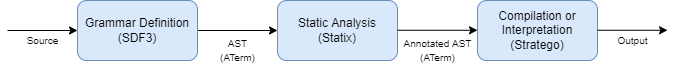
\includegraphics[width=\textwidth]{img/spoofax-p.png}}
  \caption{The Spoofax language workbench pipeline. Source code is parsed using SDF3, analyzed using Statix, then compiled or executed using Stratego.}
  \label{fig:spoofax_pipeline}
\end{figure}

\todo[inline]{improve resolution of spoofax pipeline diagram}

The Spoofax language workbench \cite{Spoofax2021} is a software suite that combines various meta-languages\footnote{A programming language that describes some aspect of another programming language.} and tools to allow users to easily design and implement (domain-specific) programming languages. Beyond parsing, static analysis, and execution, the language workbench is capable of automatically generating various IDE features including syntax highlighting, inline error markers, go-to-definition, hover annotations, and more. A standalone plugin for the Eclipse IDE providing these features can be automatically generated from a Spoofax language project.\\

The most recent stable version of Spoofax, as of the time of writing, is Spoofax 2 \cite{KatsV10}. However, work has been ongoing on Spoofax 3, which retains the same meta-languages and pipeline setup, but integrates this pipeline using PIE \cite{KonatSEV19}, a framework for incrementalizing build tasks. Using PIE, various aspects of Spoofax 3 gain support for incremental compilation "for free", leading to considerable performance gains in both the language development process, as well as the performance of the artifacts produced by the workbench. All projects discussed in this paper, particularly Tim and Dynamix, have been integrated directly into Spoofax 3.\\

The Spoofax language workbench consists of a family of meta-languages that each describe an aspect of a programming language. These meta-languages are often declarative and inspired by academic work, such that it is easy for users to get started if they are familiar with the programming languages academic field. Creating a new language using the Spoofax language workbench amounts to defining each section of the "compiler pipeline" using the appropriate meta-langauge. \Cref{fig:spoofax_pipeline} shows the current compiler pipeline for use in Spoofax. We briefly discuss each step in more detail.

\subsection{Syntax definition and parsing}
\label{sec:spoofax_parsing_aterm}
The natural first part of a language workbench is the ability to declare a grammar for the language. For this purpose, Spoofax offers the Syntax Definition Formalism 3 (SDF3) meta-language \cite{Amorim2019}. Using SDF3, a user is able to declare both lexical and context-free syntax productions for their language. From this declaration, SDF3 generates a scannerless parser with support for error recovery, a pretty-printer, and a syntax highlighter \cite{AmorimV20}.\\

\Cref{fig:sdf3_example} shows an example of an SDF3 definition for a simple arithmetic language. Two lexical sorts are defined, \texttt{INT} and \texttt{ID} which represent an integer literal and variable identifier respectively. A single context-free sort is defined, \texttt{Exp}, which represent an arbitrary expression. The distinction between lexical and context-free sorts determines is similar to that between grammar productions and lexical tokens in other parsers, and mainly determines the way in which the resulting value is represented in the AST (a lexical production yields a string of its contents, whereas a context-free production produces a tuple containing its subterms).\\

The \texttt{LAYOUT} syntax-production on line 5\todo{check/fix line numbers} is used to allow implicit layout between terms in context-free productions. Without this declaration, an expression such as \texttt{1 + 2} would be rejected as invalid. This may be surprising since the syntax for addition is defined with explicit spaces surrounding the \texttt{+} token. Indeed, SDF3 treats this declaration as \texttt{Exp LAYOUT? '+' LAYOUT? Exp}, and only uses the formatting supplied by the language author for the generated pretty-printer. \\

\todo[inline]{remove next paragraph in favor of being more brief and merging it in the previous paragraph?}
The grammar in \cref{fig:sdf3_example} is ambiguous: the expression \texttt{1 + 2 * 3} can be parsed as either \texttt{(1 + 2) * 3} or \texttt{1 + (2 * 3)}. This is resolved through the use of the \textbf{\texttt{context-free priorities}} section (line 25-26). Here, we explicitly state that the division and multiplication operators should bind more tightly than the addition and subtraction operators. Within the same precedence level, each operator is marked as left-associative by annotating its group with \texttt{left:}. The \texttt{\{bracket\}} production in line 15 allows for brackets to be used to explicitly enforce order of operations. The pretty-printer generated by SDF3 will only include these brackets in the output if they are necessary.\\

\begin{figure}
  \begin{sdf3*}{firstline=3,firstnumber=1}
module start

lexical sorts INT ID
lexical syntax
  INT = [1-9] [0-9]*
  ID = [A-Za-z] [A-Za-z0-9]*
  LAYOUT = [\ \n\r\t]

context-free sorts Exp
context-free syntax
  Exp = <(<Exp>)> {bracket}
  Exp.Add = <<Exp> + <Exp>> {left}
  Exp.Sub = <<Exp> - <Exp>> {left}
  Exp.Mul = <<Exp> * <Exp>> {left}
  Exp.Div = <<Exp> / <Exp>> {left}

  Exp.Var = <<ID>>
  Exp.Int = <<INT>>

  Exp.Let = <let <ID> = <Exp> in <Exp>>

context-free priorities
  {left: Exp.Mul Exp.Div} > {left: Exp.Add Exp.Sub} > {Exp.Let}
  \end{sdf3*}
  \caption{A simple SDF3 grammar for an arithmetic language that supports variable bindings.}
  \label{fig:sdf3_example}
\end{figure}

The parser generated by SDF3 ouputs an \ac{AST} in the \acf{ATerm}. This format originated in the ASF+SDF formalism \cite{DHP:1996}, a precursor to the Spoofax language workbench. It is a simple data transfer format that supports strings, integers, lists, tuples, tagged tuples (constructors), and annotations. The grammar for the ATerm format can be seen in \cref{gr:aterm}. \acp{ATerm} are used pervasively across the Spoofax language workbench and are supported as data format in all Spoofax meta-languages. \Cref{fig:sdf3_example_parse_output} shows an example of the parsing output for a simple program using the grammar defined in \cref{fig:sdf3_example}.\\

\begin{figure}
  \centering
  \begin{subfigure}{.35\textwidth}
    \centering
    \begin{mat}
let x = 10 in
  let y = 20 in
    let z = x + y in
      (10 + x) * y / z
    \end{mat}
  \end{subfigure}\hfill%
  \begin{subfigure}{.585\textwidth}
    \centering
    \begin{statix*}{firstline=5,lastline=20,firstnumber=1}
module main

rules
  foo(
Let(
  "x",
  Int("10"),
  Let(
    "y",
    Int("20"),
    Let(
      "z",
      Add(Var("x"), Var("y")),
      Div(
        Mul(Add(Int("10"), Var("x")), Var("y")),
        Var("z")
      )
    )
  )
)
  ).
    \end{statix*}
  \end{subfigure}
  \caption{An example expression in the arithmetic language declared in \cref{fig:sdf3_example}\protect\footnotemark. The parsed \ac{AST} in \ac{ATerm} format as produced by the generated parser can be seen on the right.}
  \label{fig:sdf3_example_parse_output}
\end{figure}

\begin{grammar}[The grammar for the \ac{ATerm} data representation format.][][gr:aterm]
  \firstcase{\prodname{term}}{\prodname{int literal}}{Integer literal}
  \otherform{\prodname{string literal}}{String literal}
  \otherform{\prodname{identifier}\textbt{(}\prodname{terms}\textbt{)}}{Constructor}
  \otherform{\textbt{[}\prodname{terms}\textbt{]}}{List literal}
  \otherform{\textbt{[}\prodname{terms}\textbt{]}}{Tuple literal}
  \otherform{\prodname{term}\textbt{\{}\prodname{terms}\textbt{\}}}{Annotated term}\\

  \firstcase{\prodname{terms}}{\epsilon}{}
  \otherform{\prodname{term}}{}
  \otherform{\prodname{term}\textbt{, }\prodname{terms}}{}\\

  \firstcase{\prodname{int literal}}{\texttt{'-'? [1-9] [0-9]*}}{}
  \firstcase{\prodname{string literal}}{\textbt{" }\prodname{string char}\textbt{* "}}{}
  \firstcase{\prodname{identifier}}{\texttt{[A-Za-z] [A-Za-z0-9.\_-]*}}{}
\end{grammar}

\todo{ensure footnote on correct page}
\footnotetext{The syntax highlighting in this snippet is exactly the syntax highlighting that SDF3 automatically generates using the grammar definition.}

Spoofax will automatically derive an \textit{algebraic signature} from all SDF3 declarations. Such a signature dictates the exact structure that an \ac{ATerm} expression can take such that it is a valid AST\footnote{Here, valid \ac{AST} means that it is an \ac{AST} that can be produced by the parser (i.e. it has a lexical equivalent), and not necessarily that this \ac{AST} is valid according to the static and dynamic semantics of the language.}. These signatures are used by various other meta-languages in the Spoofax language workbench to provide better static analysis features. \Cref{fig:sdf3_example_signature} shows the signature for the example grammar in both formal and Spoofax syntax formats.\\

% For some reason this "centers" the algebraic signature and the statix signature.
\newsavebox{\sdfsignaturebox}
\begin{lrbox}{\sdfsignaturebox}\begin{minipage}{.45\textwidth}
\begin{statix*}{firstline=3,firstnumber=1}
module main

signature
  sorts
    INT = string
    ID = string
    Exp

  constructors
    Add : Exp * Exp -> Exp
    Sub : Exp * Exp -> Exp
    Mul : Exp * Exp -> Exp
    Div : Exp * Exp -> Exp
    Var : ID -> Exp
    Int : INT -> Exp
    Let : ID * Exp * Exp -> Exp
\end{statix*}
\end{minipage}
\end{lrbox}

\begin{figure}
  \centering
  \begin{subfigure}{.45\textwidth}
    \centering
    \usebox{\sdfsignaturebox}
  \end{subfigure}\hfill%
  \begin{subfigure}{.5\textwidth}
    \centering
    $$ S = \{\texttt{INT}, \texttt{ID}, \texttt{Exp}\} $$
    \begin{equation*}
    \begin{aligned}
    \Sigma = \{ \; & \texttt{Add} : \texttt{Exp} \times \texttt{Exp} \to \texttt{Exp}, \\
                  & \texttt{Sub} : \texttt{Exp} \times \texttt{Exp} \to \texttt{Exp}, \\
                  & \texttt{Mul} : \texttt{Exp} \times \texttt{Exp} \to \texttt{Exp}, \\
                  & \texttt{Div} : \texttt{Exp} \times \texttt{Exp} \to \texttt{Exp}, \\
                  & \texttt{Var} : \texttt{ID} \to \texttt{Exp}, \\
                  & \texttt{Int} : \texttt{INT} \to \texttt{Exp}, \\
                  & \texttt{Let} : \texttt{ID} \times \texttt{Exp} \times \texttt{Exp} \to \texttt{Exp} \; \}
    \end{aligned}
    \end{equation*}
  \end{subfigure}
  \caption{The algebraic signature for the grammar in \Cref{fig:sdf3_example}. Left shows the signature of the grammar defined in the Statix meta-language, right shows the grammar in equivalent formal term algebra notation. The left source is automatically derived from the grammar definition by SDF3 as part of the compilation process.}
  \label{fig:sdf3_example_signature}
\end{figure}

Other features that SDF3 offers include the ability to specify layout constraints for grammar productions (often crucial for languages that have significant whitespace such as Python and Haskell) and automatic error recovery and placeholder insertion (needed for robust autocomplete). For more information on SDF3 and parsing within the Spoofax language workbench, the reader is invited to consult the relevant academic work, particularly the work by Visser et al. across various papers \cite{KatsV10a, Spoofax2021, Amorim2019, AmorimV20,KallebergV07, WachsmuthKV14}.

\subsection{Static analysis with constraint solvers}
\label{sec:spoofax_constraint}
The current meta-language used for static analysis in the Spoofax workbench is Statix \cite{AntwerpenPRV18}. Statix is a declarative language that performs static analysis through the use of constraints. A Statix specification consists of a set of declarative rules that specify constraints that should hold for a program to be valid. If the Statix logic solver can find a solution for which all constraints hold for a given input \ac{AST}, a program is considered well-typed. Name binding correctness is asserted through the use of \textit{scope graphs} \cite{TUD-SERG-2015-009}, although their exact semantics are beyond the scope of this paper. The reader is referred to the work by van Antwerpen et al. \cite{TUD-SERG-2015-009,AntwerpenPRV18,VanAntwerpen2016} should they be interested in their exact workings. \\

\Cref{fig:stx_example} shows an example typing rule in both formal notation and Statix syntax. The \texttt{typeOfExpression} rule and $\Gamma \vdash v : \texttt{T}$ notation are equivalent, in that they both describe the relationship between an expression and its type. Within the \textit{head} of the Statix rule, the \texttt{Div(a, b)} node is pattern-matching on exactly the \ac{ATerm} that is output by the parser. Indeed, all values in Statix (including the \texttt{INT()} term) are \acp{ATerm}. Using the signatures generated by SDF3 (see \cref{sec:spoofax_parsing_aterm}, \cref{fig:sdf3_example_signature}), the Statix meta-language can statically ensure that these pattern-matching operations are valid.\\

Beyond simply indicating whether some input \ac{AST} is valid according to the Statix specification, the Statix solver also allows users to attach \textit{properties} to arbitary AST nodes. These properties are arbitrary \ac{ATerm} values and can later be read from outside Statix. Common properties used in Statix specifications are the \texttt{ref} and \texttt{type} properties, which represent the declaring node and the type of a node respectively. The Spoofax language workbench has built-in support for reading the values of these two properties to provide editor services such as hover hints and go-to-definition. An example of the \texttt{type} annotation, as well as the tooltip generated as a result, can be seen in \cref{fig:stx_property_example}. It is worth noting that both the \texttt{type} and \texttt{ref} properties are simply conventions. A user is able to assign arbitrary properties to a property, and can read these values from other meta-languages within the Spoofax language workbench.

\begin{figure}
  \centering
  \begin{subfigure}{.55\textwidth}
    \centering
    \begin{statix*}{firstline=3,firstnumber=1}
module main

rules
  typeOfExpression(s, Div(a, b)) = INT() :-
    typeOfExpression(s, a) == INT(),
    typeOfExpression(s, b) == INT().
    \end{statix*}
  \end{subfigure}\hfill%
  \begin{subfigure}{.45\textwidth}
    \centering
    \begin{prooftree}
    \AxiomC{$\Gamma \vdash a : \texttt{INT}$}
    \noLine
    \UnaryInfC{$\Gamma \vdash b : \texttt{INT}$}
    \RightLabel{T-Division}
    \UnaryInfC{$\Gamma \vdash a \mathbin{/} b : \texttt{INT}$}
    \end{prooftree}
  \end{subfigure}
  \caption{An example typing rule for integer division in both Statix notation and formal notation. Here \texttt{s} and $\Gamma$ are analogous and correspond to the context in which the expression appears. Other rules, such as the type of an integer literal, are omitted.}
  \label{fig:stx_example}
\end{figure}

\begin{figure}
  \centering
  \begin{subfigure}{.55\textwidth}
    \centering
    \begin{statix*}{firstline=3,firstnumber=1,highlightlines={5}}
module main

rules
  typeOfExpression(s, n@Div(a, b)) = INT() :-
    typeOfExpression(s, a) == INT(),
    typeOfExpression(s, b) == INT(),
    @n.type := INT().
    \end{statix*}
  \end{subfigure}\hfill%
  \begin{subfigure}{.40\textwidth}
    \centering
    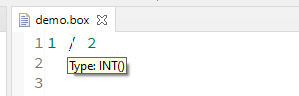
\includegraphics{img/stx_hover_example.png}
  \end{subfigure}
  \caption{An example showing the ability to attach properties to nodes in Statix. The highlighted line (left) sets the \texttt{type} property on the AST node representing the division expression. This value is later read by Spoofax to provide editor services such as hover information (right).}
  \label{fig:stx_property_example}
\end{figure}

\subsection{Transformations with Stratego}
\label{sec:spoofax_transform}
Finally, we will briefly discuss the Stratego transformation language \cite{Visser05-SCAM}. Unlike SDF3 or Statix, Stratego is more of a general imperative programming language centered around the concept of transformations, instead of a (hyper-specialized) meta-language. As a result, it generally functions as a general purpose language that, while traditionally used for interpreteration or compilation at the end of the Spoofax pipeline, may also appear between other stages to perform intermediate transformations.\\

An example of a simple Stratego program can be seen in \cref{fig:str_example}. Pattern-matching is performed on input terms, with matches transformed accordingly. The data format in use for Stratego is again the \ac{ATerm} format, with additional static analysis provided using the algebraic signature automatically derived from the SDF3 grammar.\\

\begin{figure}
  \begin{stratego*}{firstline=3,firstnumber=1}
module start

rules
  fold = innermost(fold-term)

  fold-term: Add(Int(a), Int(b)) -> Int(<addS> (a, b))
  fold-term: Sub(Int(a), Int(b)) -> Int(<subtS> (a, b))
  fold-term: Mul(Int(a), Int(b)) -> Int(<mulS> (a, b))
  fold-term: Div(Int(a), Int(b)) -> Int(<divS> (a, b))

  fold-term: Eq(Int(a), Int(a)) -> Int("1")
  fold-term: Eq(Int(a), Int(b)) -> Int("0") where not(<eq> (a, b))
  \end{stratego*}
  \caption{A simple Stratego program that performs constant folding in an arithmetic language. The \texttt{fold} strategy will apply the \texttt{fold-term} strategy until a fixpoint is reached.}
  \label{fig:str_example}
\end{figure}

\begin{figure}
  \begin{stratego*}{firstline=3,firstnumber=1}
module start

imports
  statix/api

rules
  compile-expr: n@Add(a, b) -> <compile-int-addition> (a, b)
    where a := <stx-get-ast-analysis> n; INT() := <stx-get-ast-type(|a)> n
  
  compile-expr: n@Add(a, b) -> <compile-string-concatenation> (a, b)
    where a := <stx-get-ast-analysis> n; STRING() := <stx-get-ast-type(|a)> n
  \end{stratego*}
  \caption{Many Spoofax meta-languages expose Stratego APIs. Here, the result of a Statix analysis is used to emit integer addition or string concatenation based on the type of the expression.}
  \label{fig:str_stx_example}
\end{figure}

Due to its general nature, many Spoofax features and meta-languages offer a Stratego API. This allows Stratego strategies to interact with other parts of the Spoofax workbench, such as the ability to query the results of static analysis. Consider the example in \cref{fig:str_stx_example}, which uses Statix APIs to distinguish between integer addition and string concatenation, both of which are syntactically represented as \texttt{Add(a, b)}.\\

We will further discuss Stratego and its semantics when we introduce the mini-Stratego case study in \cref{ch:case_studies}. Readers interested in learning more about Stratego and its term rewriting paradigm are encouraged to read the appropriate work by Visser et al. \cite{KallebergV07,Visser05-SCAM}.

\section{Dynamic semantics in Spoofax}
\label{sec:background_spoofax_dynamics}
\todo[inline]{rename section/something with history?}
As already briefly alluded to, Dynamix is not the first attempt at adding dynamic semantics support to the Spoofax language workbench. In fact, several projects, including some under the Dynamix name, predate the work done in this thesis.\\

The first effort at implementing dynamic semantics in the Spoofax language workbench was the DynSem meta language \cite{VerguNV15}. DynSem was conceived with goals similar to Dynamix, but was intentionally designed to mimic the notation often used by big-step operational semantics. The DynSem compiler converts such a specification into an interpreter for the language written in Java. An example of a DynSem specification can be seen in \cref{fig:dynsem_example}. We further discuss DynSem as part of the related work section in \cref{ch:related_work}.\\

\begin{figure}
  \begin{dynsem*}{firstline=3,firstnumber=1}
module start

rules
  Lit(s) --> NumV(parseI(s)).

  Plus(e1, e2) --> NumV(addI(i1, i2))
  where
    e1 --> NumV(i1);
    e2 --> NumV(i2).

  Ifz(NumV(ci), e1, e2) --> v
  where
    case ci of {
      0 => e1 --> v
      otherwise => e2 --> v
    }.
  \end{dynsem*}
  \caption{An example of a specification written using the DynSem meta-language \cite{VerguNV15}. The \texttt{-->} "arrow" is intended to be analogous to a Kahn-style big-step evaluation relation. }
  \label{fig:dynsem_example}
\end{figure}

One of the main problems with DynSem\todo{check with andrew if this is right} was that certain language constructs were hard, or even impossible, to represent in the language. Especially non-linear control flow, such as exceptions and generators, require non-trivial boilerplate in virtually every rule. Additionally, the generated interpreter is not particularly performant. While this performance has been greatly increased in follow-up work by Vergu et al. \cite{VerguV18}, they note that the generated interpreter still performed a factor of 4 slower than a hand-written interpreter for the same language. As a result of these two main drawbacks, the DynSem language saw little use within the Spoofax workbench and was eventually deprecated.\\

In an effort to remedy these issues, the Dynamix meta-language\footnote{Not to be confused with the Dynamix language presented in this paper. With the exception of this section, the term Dynamix will always refer to the language presented in this paper.} was conceived as part of Chiel Bruin's master's thesis \cite{Bruin2020}. Inspired by DynSem, the Dynamix language was conceived as a dynamic specification meta-language compatible with the semantics of the "Roger" target language, introduced in the same thesis. Unfortunately, the Roger language and corresponding FrameVM did not see any future use beyond Bruin's thesis.\todo{mention brams thesis?}\\

Despite this, the Dynamix language seemed promising. In late 2020, Eelco Visser and Andrew Tolmach started exploratory work on "Dynamix V2". The intent was to retain most of the Dynamix language, but to compile to a new continuation-based target language. If the resulting target language was able to be efficiently compiled or interpreted, this approach could resolve the runtime performance issues that DynSem suffered from. DynSem's other main problem, that of control flow, could also be resolved by using continuations, as evident from Bruin's work.\\

The Dynamix language discussed in this thesis\footnote{Dynamix as presented in this paper should really be called Dynamix v2.5. However, since the version of Dynamix designed by Bruin never made it into the Spoofax language workbench, the Dynamix presented in this paper is the first publicly usable iteration of the meta-language. In order to avoid potential confusion for Spoofax users, we decided that it would be more appropriate to call the language Dynamix, without a version number.} is a spiritual successor to these efforts by Visser and Tolmach. Many components were revamped in order to generalize their experimental prototype to a large array of languages and programming paradigms, and to fully integrate the resulting product in the Spoofax language workbench. The remainder of this thesis discusses these efforts and shows that the resulting meta-language is indeed capable of resolving many of DynSem's original issues. We should stress that no previous knowledge of the Dynamix meta-language as it appeared in Bruin's thesis is required: we will introduce the language from scratch.